\documentclass[11pt, a4paper]{report}
\usepackage[utf8]{inputenc}%codification of the document
\usepackage[french]{babel}
\usepackage{geometry}
\usepackage{times}
\usepackage{graphicx}
\usepackage{multicol}
\usepackage{float}
\usepackage{subcaption}
\usepackage{comment}
\usepackage{hyperref}
\usepackage{listings}
\usepackage{color}
\usepackage[dvipsnames]{xcolor}
\definecolor{EnoncerQuestions}{RGB}{10, 84, 68}
\definecolor{EnincerExercice}{RGB}{158, 19, 24}

\definecolor{lightgray}{rgb}{.98,.98,.98}
\definecolor{darkgray}{rgb}{.4,.4,.4}
\definecolor{blue}{rgb}{0.5, 0.2, 0.82}
\definecolor{purple}{rgb}{0.7, 0, 0.6}

\lstdefinelanguage{C}{
	keywords={typeof, new, true, false, catch, function, return, null, catch, switch, var, if, in, while, do, else, case, break},
	keywordstyle=\color{blue}\bfseries,
	ndkeywords={class, export, boolean, throw, implements, import, this},
	ndkeywordstyle=\color{darkgray}\bfseries,
	identifierstyle=\color{black},
	sensitive=false,
	comment=[l]{//},
	morecomment=[s]{/*}{*/},
	commentstyle=\color{blue}\ttfamily,
	stringstyle=\color{purple}\ttfamily,
	morestring=[b]',
	morestring=[b]"
}

\lstset{
	language=C,
	backgroundcolor=\color{lightgray},
	extendedchars=true,
	basicstyle=\footnotesize\ttfamily,
	showstringspaces=false,
	showspaces=false,
	numbers=left,
	numberstyle=\footnotesize,
	numbersep=9pt,
	tabsize=2,
	breaklines=true,
	showtabs=false,
	captionpos=b
}
\author{Badmavasan KIROUCHENASSAMY \& Caroline SCHMID}
\date{}
\title{Projet tutoré de Structures de Données - Graphes et Combinatoires : Problème du flot maximum}
\begin{document}
	\pagenumbering{roman}
	\begin{titlepage}
		\begin{center}

			\vspace*{1cm}

			\begin{figure}[h]
				\centering
				
\includegraphics[width=0.4\textwidth]{images/LOGO_Polytech-lille.jpg}
				\hspace{2cm}
				
\includegraphics[width=0.4\textwidth]{images/logo_ulille_transparent.png}
			\end{figure}

			\vspace*{2cm}

			\rule{1\textwidth}{.8pt}

			\LARGE{\textsc{Projet tutoré de Structures de Données \\-\\ Graphes et Combinatoires}}

			\vspace*{1cm}

			\LARGE{\textsc{Problème du flot maximum}}
			\vspace*{1cm}

			\small{IS2A3 - Lundi 31 mai 2021}

			\vspace*{0.5cm}
			\rule{1\textwidth}{.10pt}

			\vspace*{2.352cm}

			\large{\textit{Encadrante :} Clarisse DHAENENS}

			\vspace*{0.1cm}

			\large{\textit{Auteurs :} {Badmavasan KIROUCHENASSAMY\\Caroline SCHMID}}




		\end{center}

	\end{titlepage}


	%\setcounter{tocdepth}{2}
	\tableofcontents


	\chapter{Contexte du projet}
	\pagenumbering{arabic}
	Pour résoudre un problème de flot maximum, plusieurs algorithmes peuvent être mis en œuvre. Nous étudions ici la mise en place de l'algorithme de \textbf{DINIC} ainsi que les structures de données nécessaires et l'arborescence des fichiers.

	Le problème de flot maximum consiste à trouver le flot le plus élevé que l'on peut faire passer dans un réseau en respectant les capacités de chaque arc, soit le flot maximum que l'on peut faire passer par chaque arc.

	L'algorithme de \textbf{DINIC} permet, à partir d'un flot initial, de rechercher une chaîne améliorante dans un réseau de façon à construire un flot de valeur supérieure. En réitérant cette opération un certain nombre de fois, le flot que l'on obtient devient maximum. L'algrithme prend en paramètre un graphe d'écart, il faut donc transformer le réseau du problème de flot maximum en un graphe d'écart pour trouver le flot maximum et revenir à un réseau répondant au problème posé.

	On considère que le flot initial est de 0 et que les sommets sont numérotés de $1$ à $n$, $n$ étant le nombre de sommets.



	\chapter{Analyse}
	\section{Représentation des données}
	La chaîne améliorante de l'algorithme de \textbf{DINIC} est la chaîne du plus court chemin en nombre d'arcs et sera donc trouvée par l'algorithme de parcours en largeur. Étant donné que ce dernier algorithme génère l'arborescence donnant le plus court chemin en nombre d'arc, on l'utilise pour trouver la chaîne améliorante de l'algorithme de \textbf{DINIC}.

	L’algorithme de parcours en largeur est un algorithme parcourant le graphe par couches. Les sommets de la couche $n$ sont à une distance $n$ du sommet source. L’exploration commence donc par la source, puis ses successeurs, puis les successeurs de ses successeurs, ... jusqu’à explorer le sommet puits, on sait alors que l’on peut s’arrêter. Grâce à un tableau répertoriant les prédécesseurs des sommets marqués (par convention, le sommet prédécesseur du sommet source est lui-même), on peut retrouver le chemin le plus court en nombre d'arcs menant d’un sommet à un autre (ici, menant du sommet source au sommet puits).

	Voici le déroulement de l'algorithme de \textbf{DINIC} sur un réseau à 5 sommets et 7 arcs :
	\begin{enumerate}
		\item \verb|Réseau :|\\
	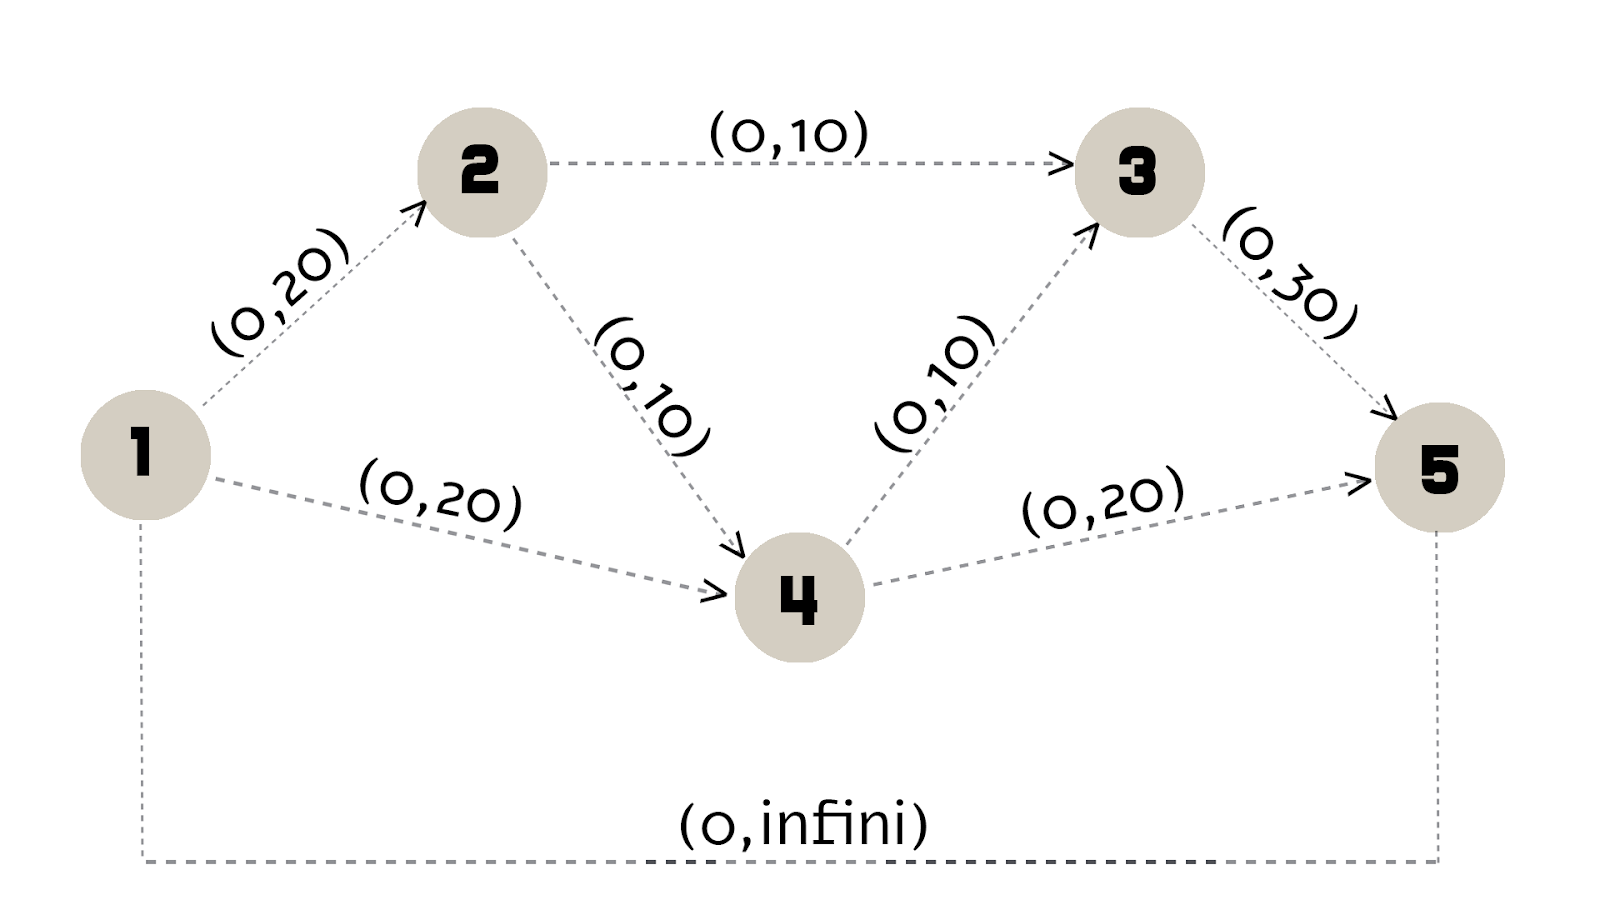
\includegraphics[width=0.7\textwidth]{images/R1.png}\\
	\pagebreak
		\item \verb|Graphe d'Écart :|\\
	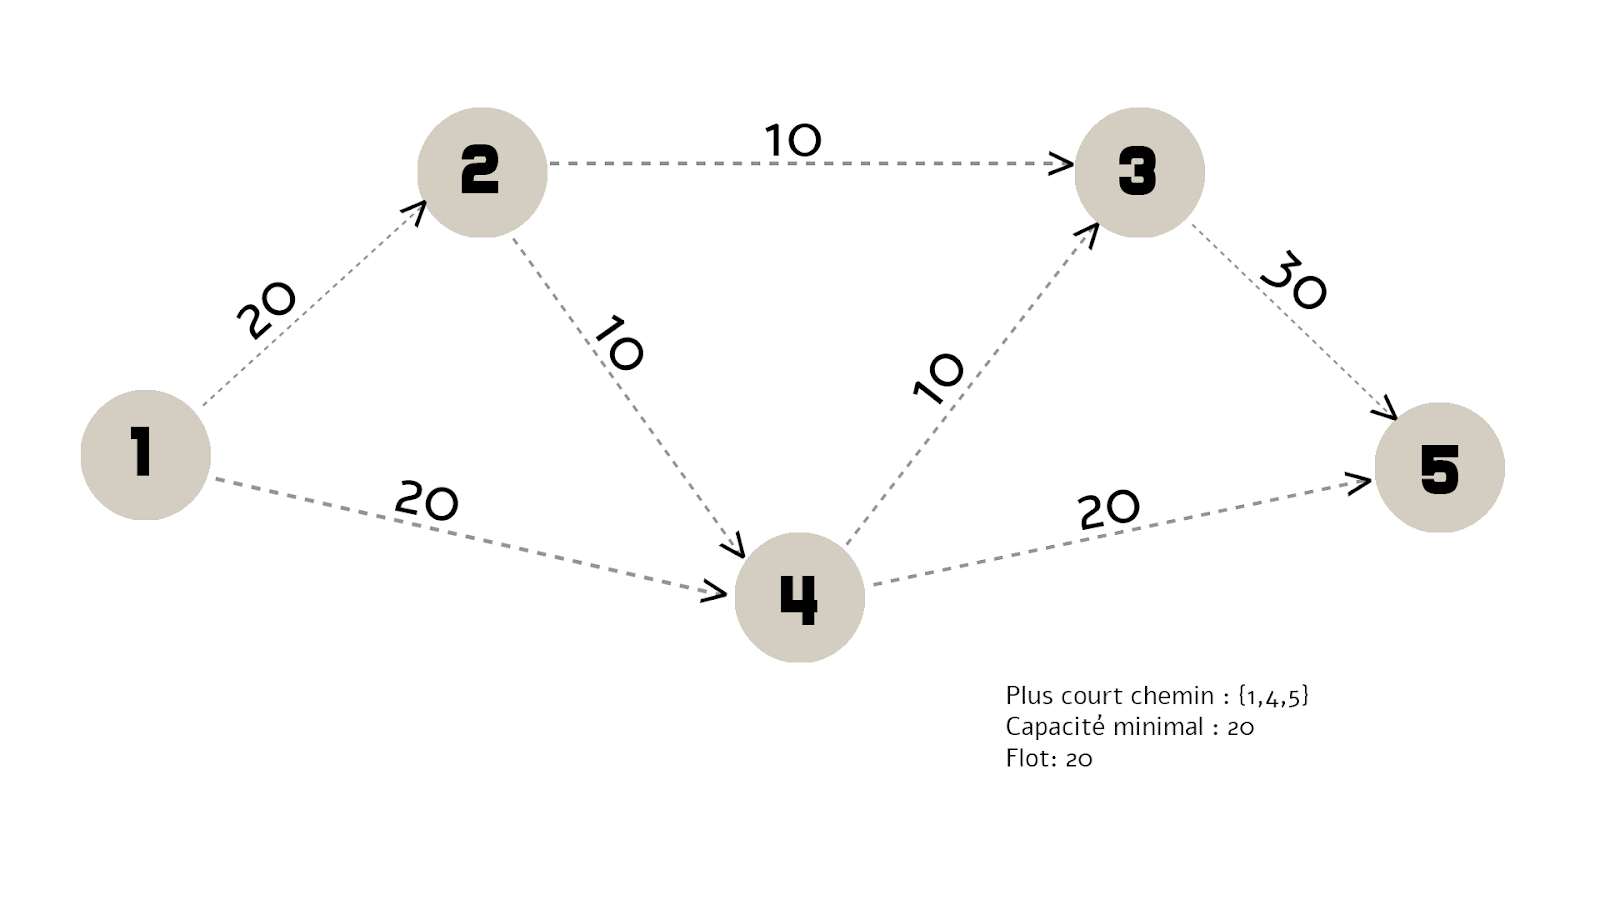
\includegraphics[width=0.7\textwidth]{images/GE1.png}\\
		\item \verb|Graphe d'Écart :|\\
	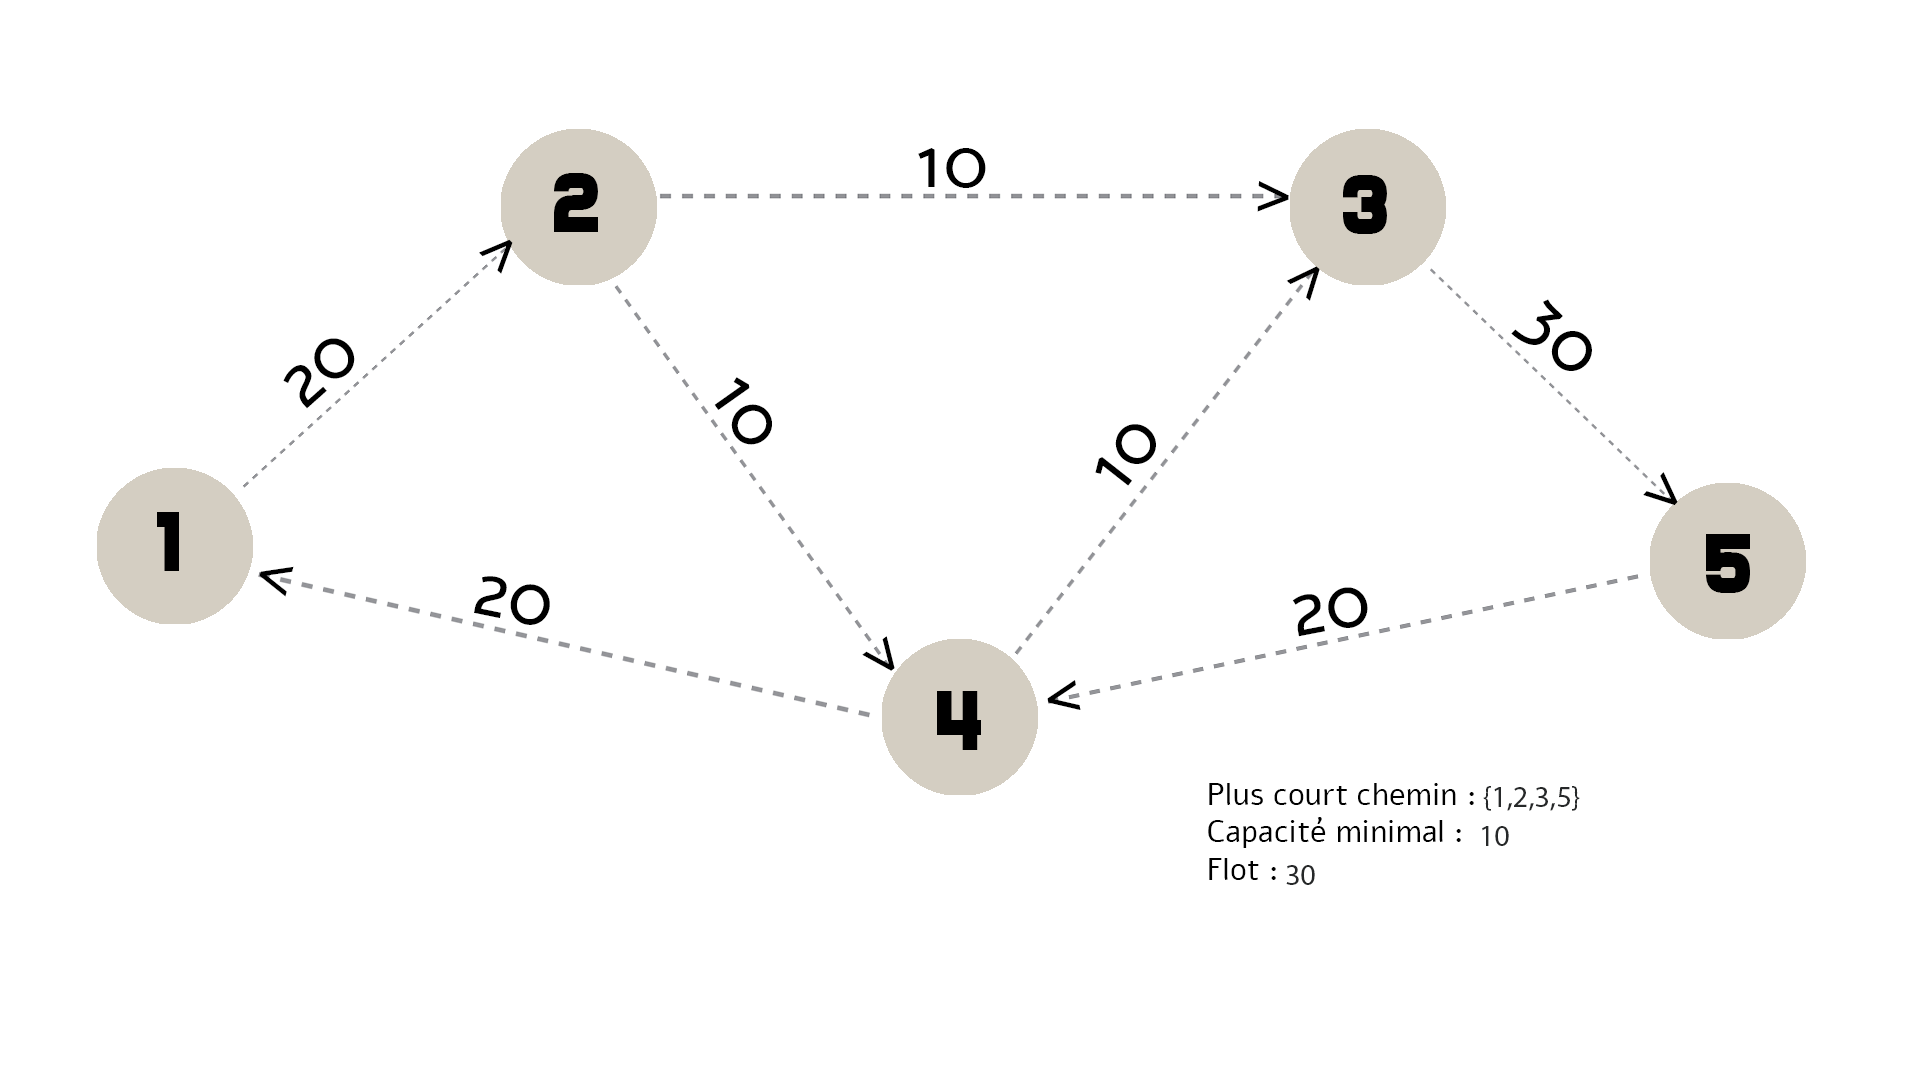
\includegraphics[width=0.7\textwidth]{images/GE2.png}\\
		\item \verb|Graphe d'Écart :|\\
	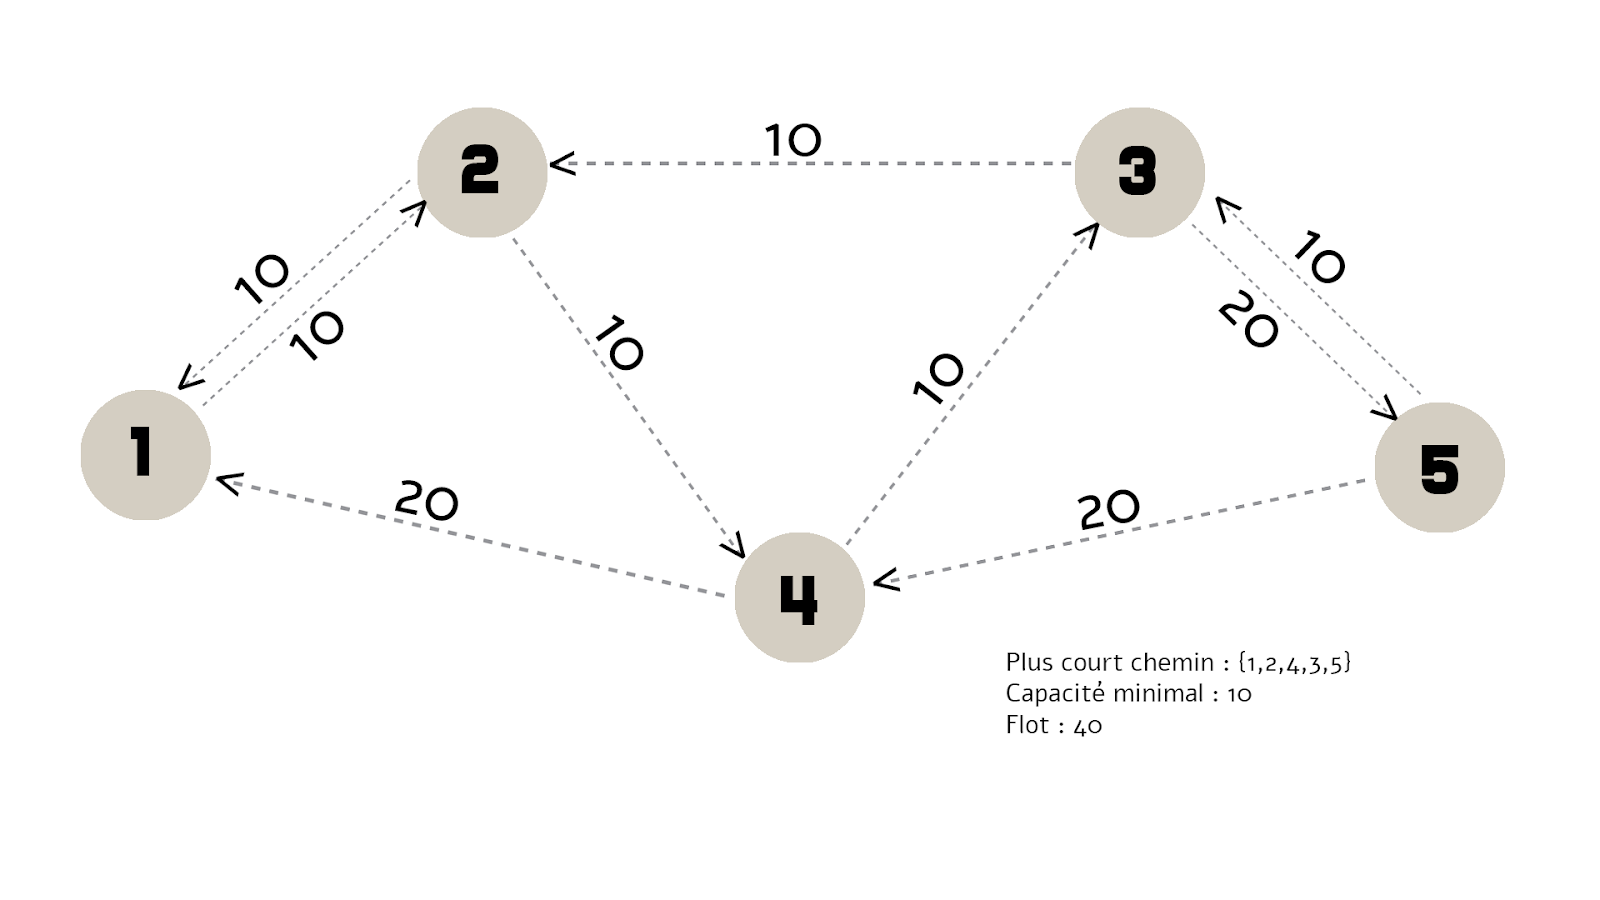
\includegraphics[width=0.7\textwidth]{images/GE3.png}\\
	\pagebreak
		\item \verb|Graphe d'Écart :|\\
	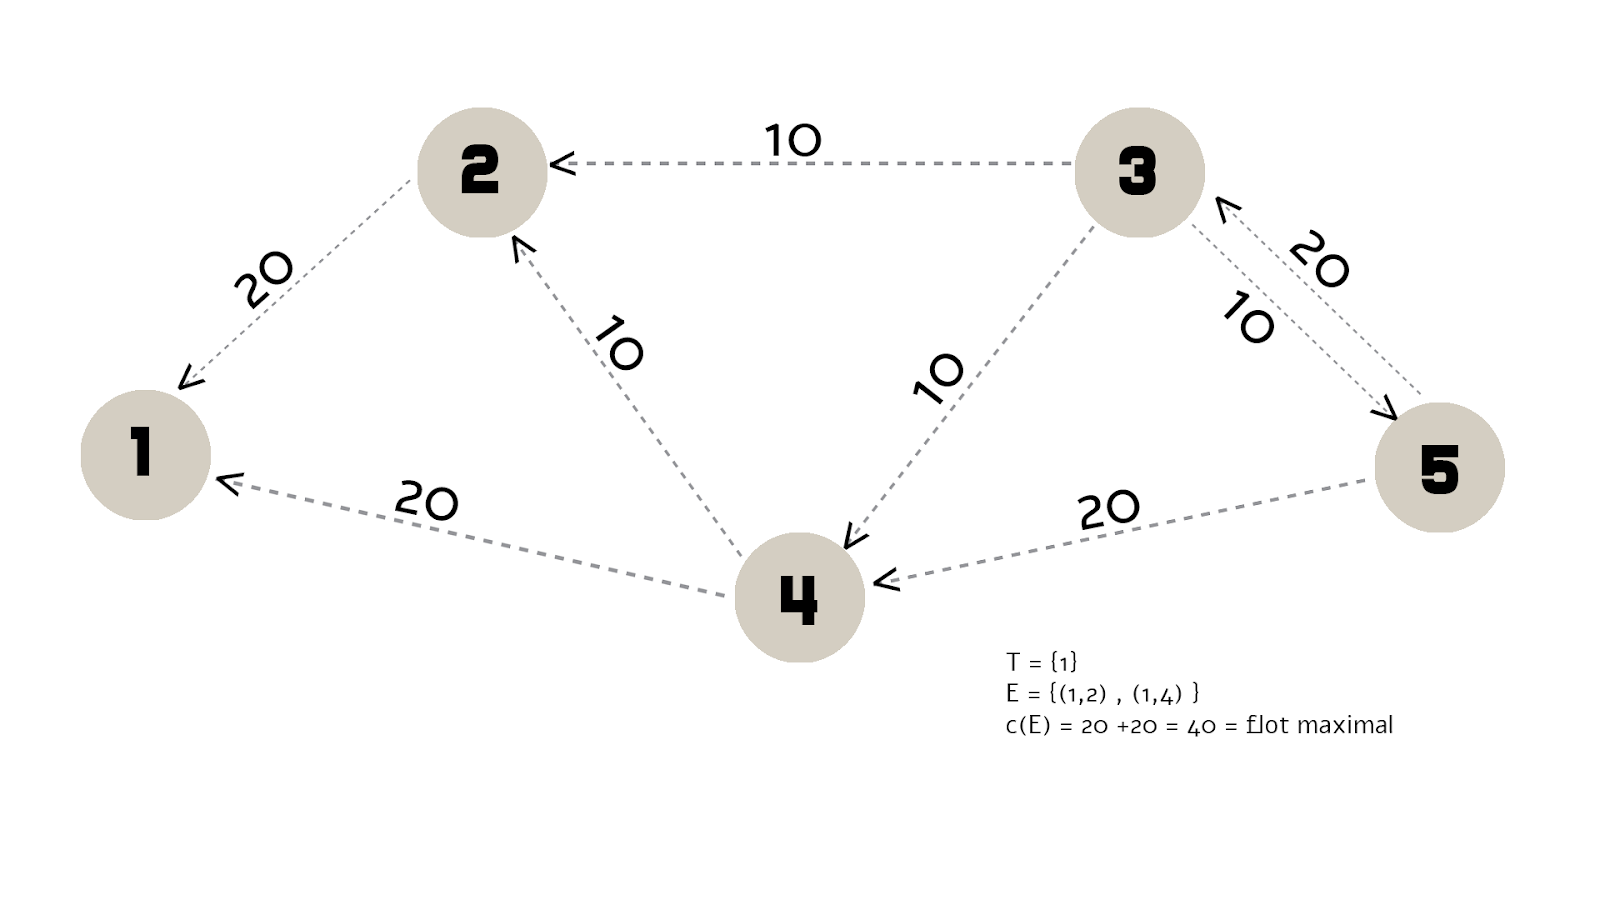
\includegraphics[width=0.7\textwidth]{images/GE4.png}\\
		\item \verb|Réseau :|\\
	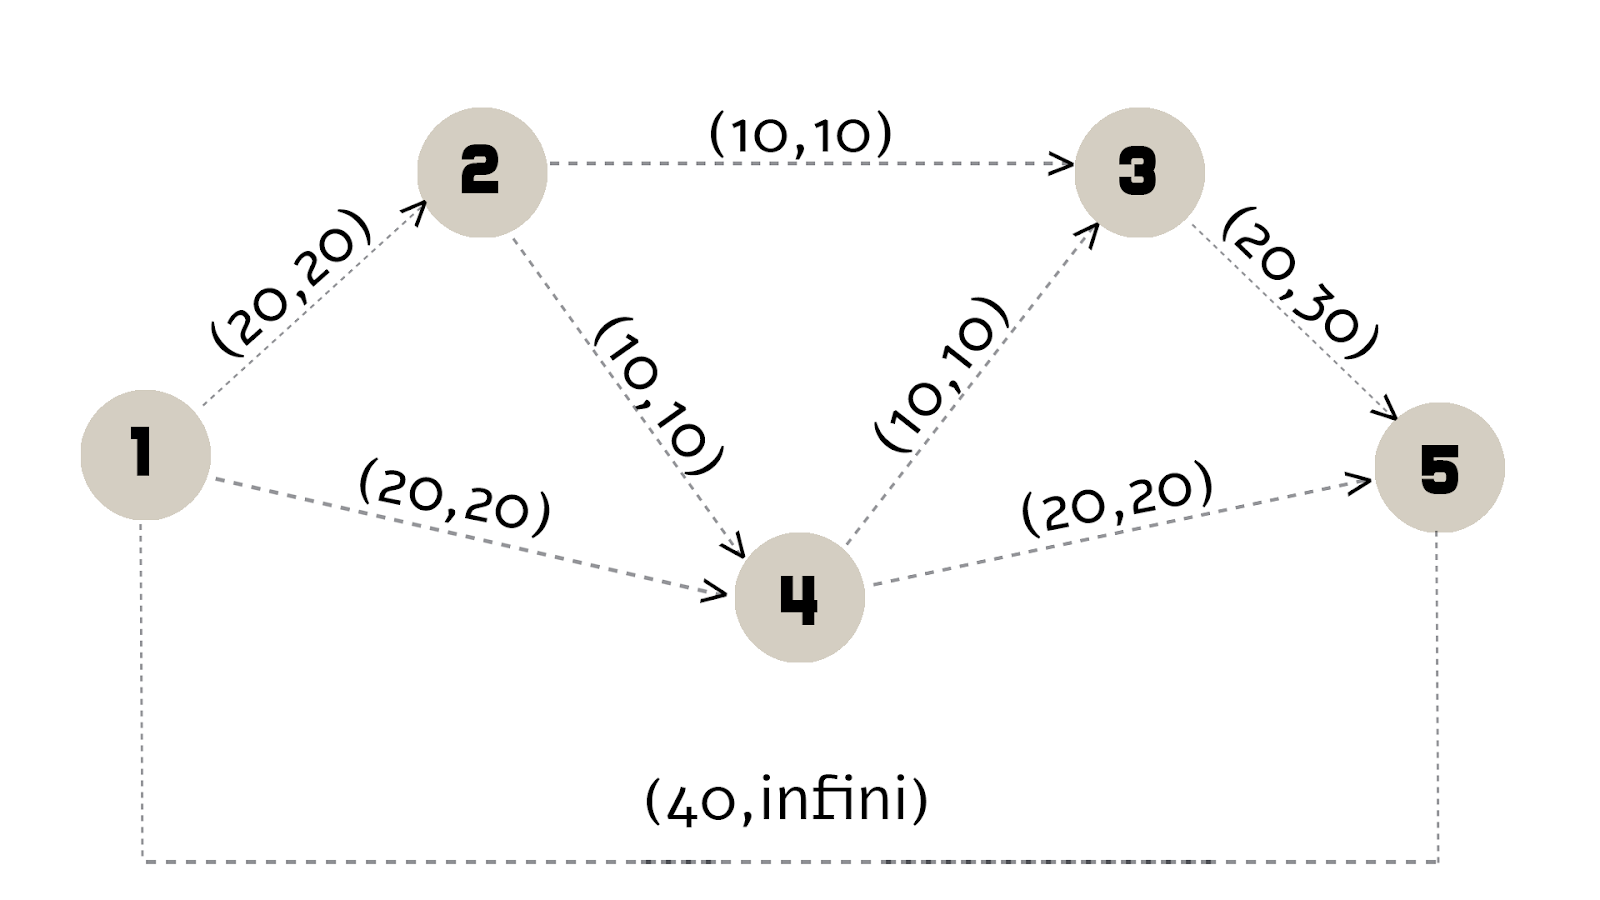
\includegraphics[width=0.7\textwidth]{images/R2.png}\\
	\end{enumerate}

	Par convention, un graphe est constitué de $n$ sommets et $m$ arcs. On utilisera donc ces notations pour alléger le texte.

	Pour représenter le réseau, on voit trois structures de données possibles. Elles seront illustrées ici par une représentation graphique basée sur l'exemple du réseau précédent, dans son état initial.

	\pagebreak
	\begin{enumerate}
		\item Une matrice d'incidence :

		Un tableau de tableaux : chaque case du premier tableau est elle-même un tableau. les sommets sont représentés en lignes et les arcs en colonnes. La case est à $0$ si le sommet n'est pas incident à l'arc, $1$ s'il est source de l'arc et $-1$ s'il est destination de l'arc.\\
		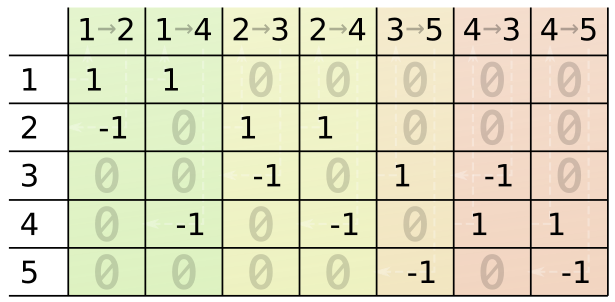
\includegraphics[width=0.7\textwidth]{images/Matrice_incidence.png}\\

		\item Un tableau sommets - successeurs :

		Deux tableaux. Le premier tableau de la longueur du nombre d'arc est un tableau de pointeurs pointant vers le premier sommet successeur dans le second tableau. Le second tableau, de la longueur du nombre d'arcs, représente les successeurs des sommets du premier tableau. Les successeurs d'un même sommet sont contigus dans le second tableau.\\
		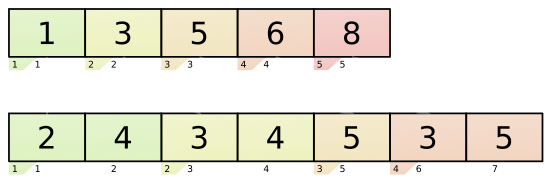
\includegraphics[width=0.7\textwidth]{images/tableau_pointeur_succ.png}\\

		\pagebreak
		\item Un tableau de listes de successeurs :

		Un tableau de listes de successeurs. Chaque case contient une liste. La tête de la liste indique quel est le sommet source et les maillons de la liste sont les successeurs de ce sommet source.\\
		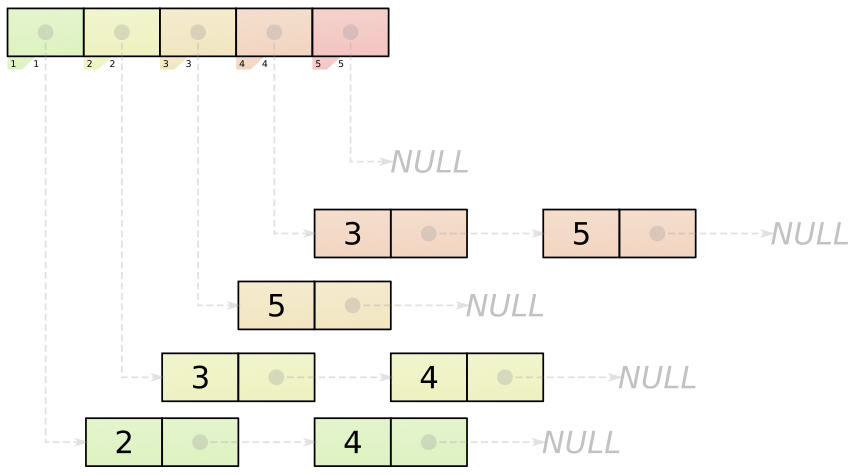
\includegraphics[width=0.8\textwidth]{images/tableau_liste_succ.png}\\

	\end{enumerate}

    Comparons les avantages des trois structures de données sur 3 critères : le coût de stockage en mémoire, le coût de traitement en accès au successeur d'un sommet donné et finalement l'ajout et la suppression d'un successeur d'un sommet donné.

    \begin{center}
        \begin{tabular}{ | p{0.15\textwidth} | p{0.3\textwidth} | p{0.3\textwidth} | p{0.3\textwidth} | }
            \hline
            	 &
            	Matrice d'incidence &
            	Tableau sommets - successeurs &
            	Tableau de listes de successeurs \\
            \hline
            	Coût de stockage en mémoire &
            	\textcolor{BrickRed}{La dimension de la matrice est de $(n \times m)$. L'initialisation du tableau occupe une taille de $(n \times m)$, donc la complexité en coût mémoire vaut $(n \times m) \times sizeof(int)$.} &
            	\textcolor{OliveGreen}{La complexité en coût mémoire de cette structure de donnée est simplement de $(n+m)$.} &
	            \textcolor{OliveGreen}{Le tableau initial est de taille $n$ et il y a $m$ maillons répartis dans les différentes listes du tableau. Ces structures sont allouées dynamiquement. La complexité en coût mémoire est de nouveau de $(n + m)$.}\\
            \hline
            	Coût de traitement en accès au successeur &
            	\textcolor{BrickRed}{Il faut parcourir la matrice afin de trouver les successeurs d'un sommet vu que c'est une matrice d'incidence donc on ne peut pas se concentrer sur une seule ligne ou colonne. La complexité est donc de\hspace{1cm} $O(n \times m)$.} &
            	\textcolor{OliveGreen}{On a directement l'indice dans le tableau de successeurs en fonction du tableau de sommets. Donc on n'a pas vraiment de traitement à effectuer. La complexité est donc de $O(n)$.} &
            	\textcolor{OliveGreen}{On a une liste chaînée donc il y a le coût de parcours des maillons. La complexité est donc de $O(n)$.}\\
            \hline
            	Ajout et suppression d'un successeur &
            	\textcolor{BrickRed}{Il faut redimensionner une matrice à 2 dimensions et donc réalouer plus ou moins de mémoire, et déplacer les données étant donné qu'elles sont stockées dans des cases contigues (principe du tableau). La complexité est en $O(n \times m)$.} &
            	\textcolor{Orange}{Le second tableau, de successeurs, doit être redimensionné, donc il faut potentiellement déplacer le tableau. La complexité de cette opération est en $O(m)$.} &
            	\textcolor{OliveGreen}{L'ajout ou la suppression d'un maillon dans une liste a un coût constant et donc négligeable. Sa complexité est en $O(1)$.}\\
            \hline
        \end{tabular}
    \end{center}

	Par ce tableau, on se rend compte que, pour le tableau sommets - successeurs et le tableau de listes de successeurs, leurs complexités sont les mêmes en stockage mémoire et en accès au successeur. Cependant, la deuxième structure de donnée à une complexité an ajout et suppression de successeurs plus faible que la première stucture de donnée. On abandonne donc l'idée d'implémenter la première structure de données. La matrice d'incidence à une complexité largement moins bonne que celle du tableau de listes de successeurs sur les différents critères. Pour résoudre le problème de maximisation de flot par l'algorithme de \textbf{DINIC}, nous allons donc utiliser la structure de données de tableau de listes de successeurs.

    Pour réduir le nombre d'ajout et de suppressions d'arcs dans le graphe d'écart, lors de ses mises à jour entre deux itérations de \textbf{DINIC}, on pourrait, lors de la création du graphe à partir du réseau, créer pour chaque sommet dans le graphe un arc avec le flot égalant la capacité de l'arc du graphe et un arc inverse de flot nul. Ça permettrait d'utiliser les arcs déjà construits et de ne pas ajouter de nouvel arc ou d'en retirer un de flot nul.

    Nous n'appliquerons pas cette idée car elle utilise beaucoup d'espace mémoire souvent inutil. L'espace économisé n'est pas nécessairement important, mais il devient significatif lorsque le nombre d'arcs devient grand car on passe approximativement de $m$ arcs à $2 \times m$ arcs. On notera que cette solution aurait pu être appliquée au tableau sommets - successeurs et il n'y aurait plus eu d'avantages à utiliser la soulution retenue plutôt que cette structure de données avec $2 \times m$ arcs pour les deux structures de données.

    L'ordre d'apparition des successeurs dans la liste des successeurs n'importe pas, les structures de données ne tiendront donc pas compte de l'ordre alpha-numérique.

	\section{Implémentation de la structure de données choisie}

	Pour dérouler l'algorithme de \textbf{DINIC} et trouver le flot maximum du réseau donné, on utilisera 4 structures de données :
	\begin{enumerate}
		\item Une liste, et ses maillons, représentant les successeurs d'un sommet dans le réseau (listes constituant le tableau de listes de successeurs).
		\item Une liste, et ses maillons, représentant les successeurs d'un sommet dans le graphe d'écart (listes constituant le tableau de listes de successeurs).
		\item Une liste, et ses maillons, représentant les sommets constituant le plus court chemin en nombre d'arcs permettant d'améliorer le flot d'un graphe donné.
		\item Une file permettant de trouver le plus court chemin en nombre d'arcs dans un graphe donné.
	\end{enumerate}

	Voici le code $C$ décrivant ces structures de données :
	\lstset{language=C}
	\begin{lstlisting}
        /* Reseau */

        struct maillon_graph_reseau {
            int id;
            int flot;
            int capacite;
            struct maillon_graph_reseau* next;
        };

        struct liste_graph_reseau {
            int id;
            struct maillon_graph_reseau* head;
        };



        /* Graphe Ecart */

        struct maillon_graph_ecart {
            int id;
            int flot_entrant;
            struct maillon_graph_ecart* next;
        };

        struct liste_graph_ecart {
            int id;
            struct maillon_graph_ecart* head;
        };



        /* Chemin */

        struct maillon_chemin {
            int id;
            int capacite_residual;
            struct maillon_chemin * next;
        };

        struct liste_chemin {
            struct maillon_chemin * head;
        };



        /* File */

        struct file {
            int* tab;
            int taille;
            int read_end;
            int write_end;
            int n;
        };
	\end{lstlisting}

	Lorsqu'un maillon est le dernier de la liste, il pointe vers un pointeur null de son type :

	\lstset{language=C}
	\begin{lstlisting}
        /* Reseau */

        #define NIL_lr (struct liste_graph_reseau*) 0
        #define NIL_mr (struct maillon_graph_reseau*) 0



        /* Graphe Ecart */

        #define NIL_lge (struct liste_graph_ecart *) 0
        #define NIL_mge (struct maillon_graph_ecart *) 0



        /* Chemin */

        #define NIL_lc (struct liste_chemin *) 0
        #define NIL_mc (struct maillon_chemin *) 0
	\end{lstlisting}

	\pagebreak
	De manière schématique, sur un exemple donné ci-dessous, les structures de données ressembleraient donc à :\\
	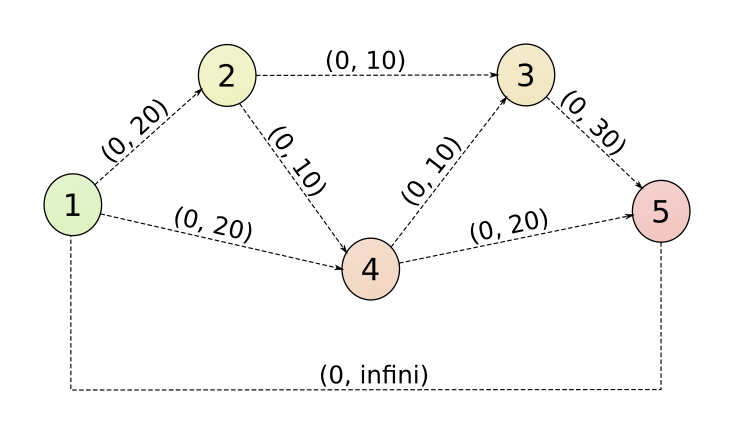
\includegraphics[width=0.7\textwidth]{images/R3.png}\\
	\begin{itemize}
        \item Réseau : le réseau initial :\\
		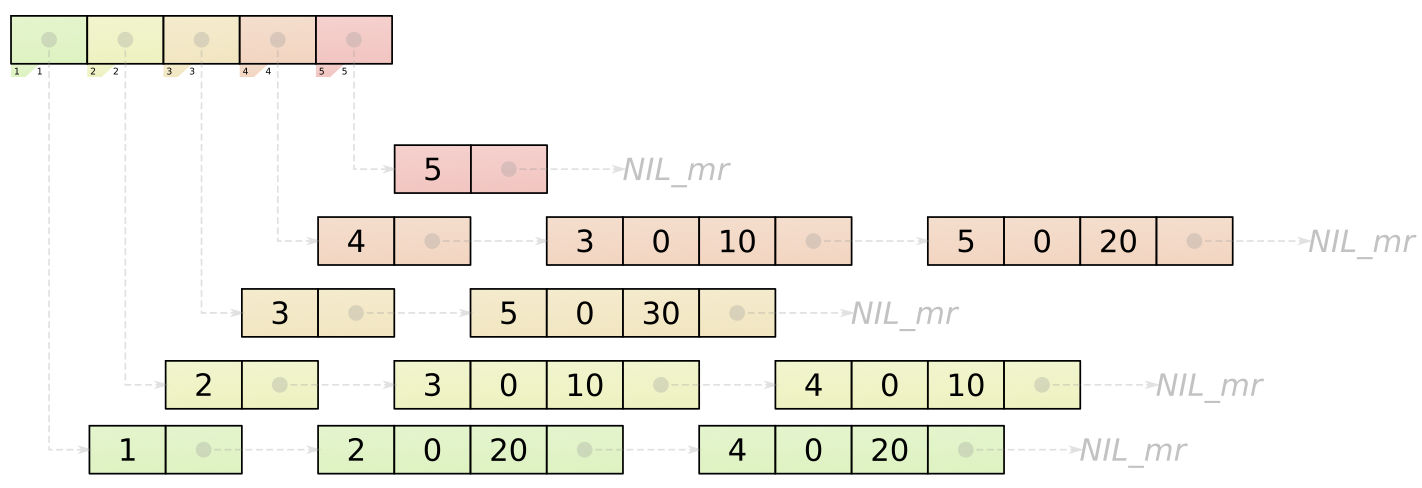
\includegraphics[width=0.8\textwidth]{images/sch_reseau.png}\\

        \item Graphe Écart : le premier graphe d'écart construit à partir du réseau :\\
		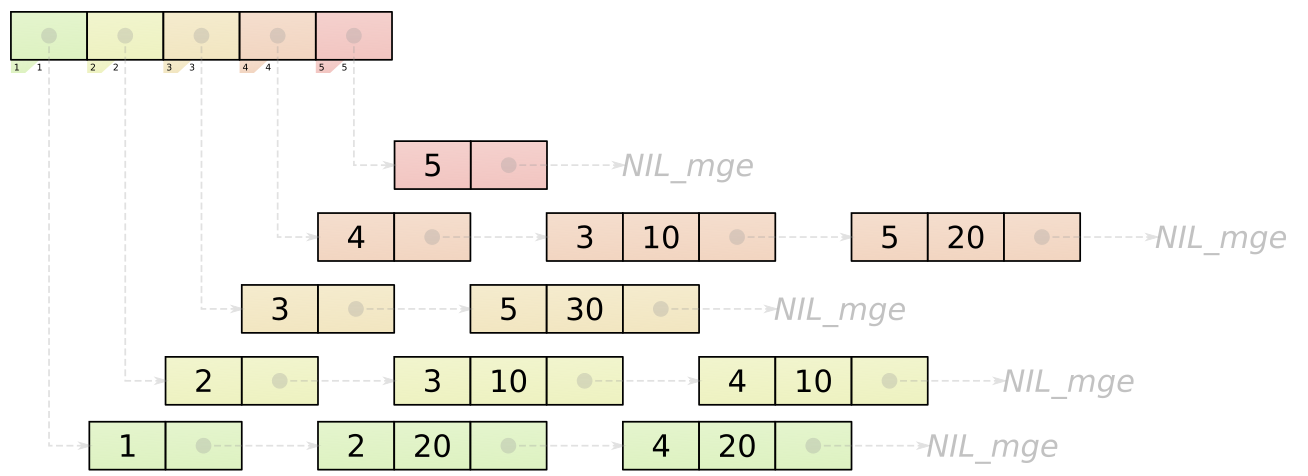
\includegraphics[width=0.8\textwidth]{images/sch_graphe_ecart.png}\\

        \item Chemin : le premier chemin améliorant :\\
		
\includegraphics[width=0.7\textwidth]{images/sch_chemin.png}\\

		\pagebreak
        \item File : la file à la fin de la construction du premier chemin améliorant :\\
		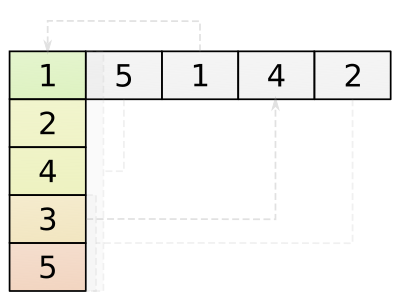
\includegraphics[width=0.25\textwidth]{images/sch_file.png}\\
	\end{itemize}

	L'arborescence des fichiers est la suivante :

	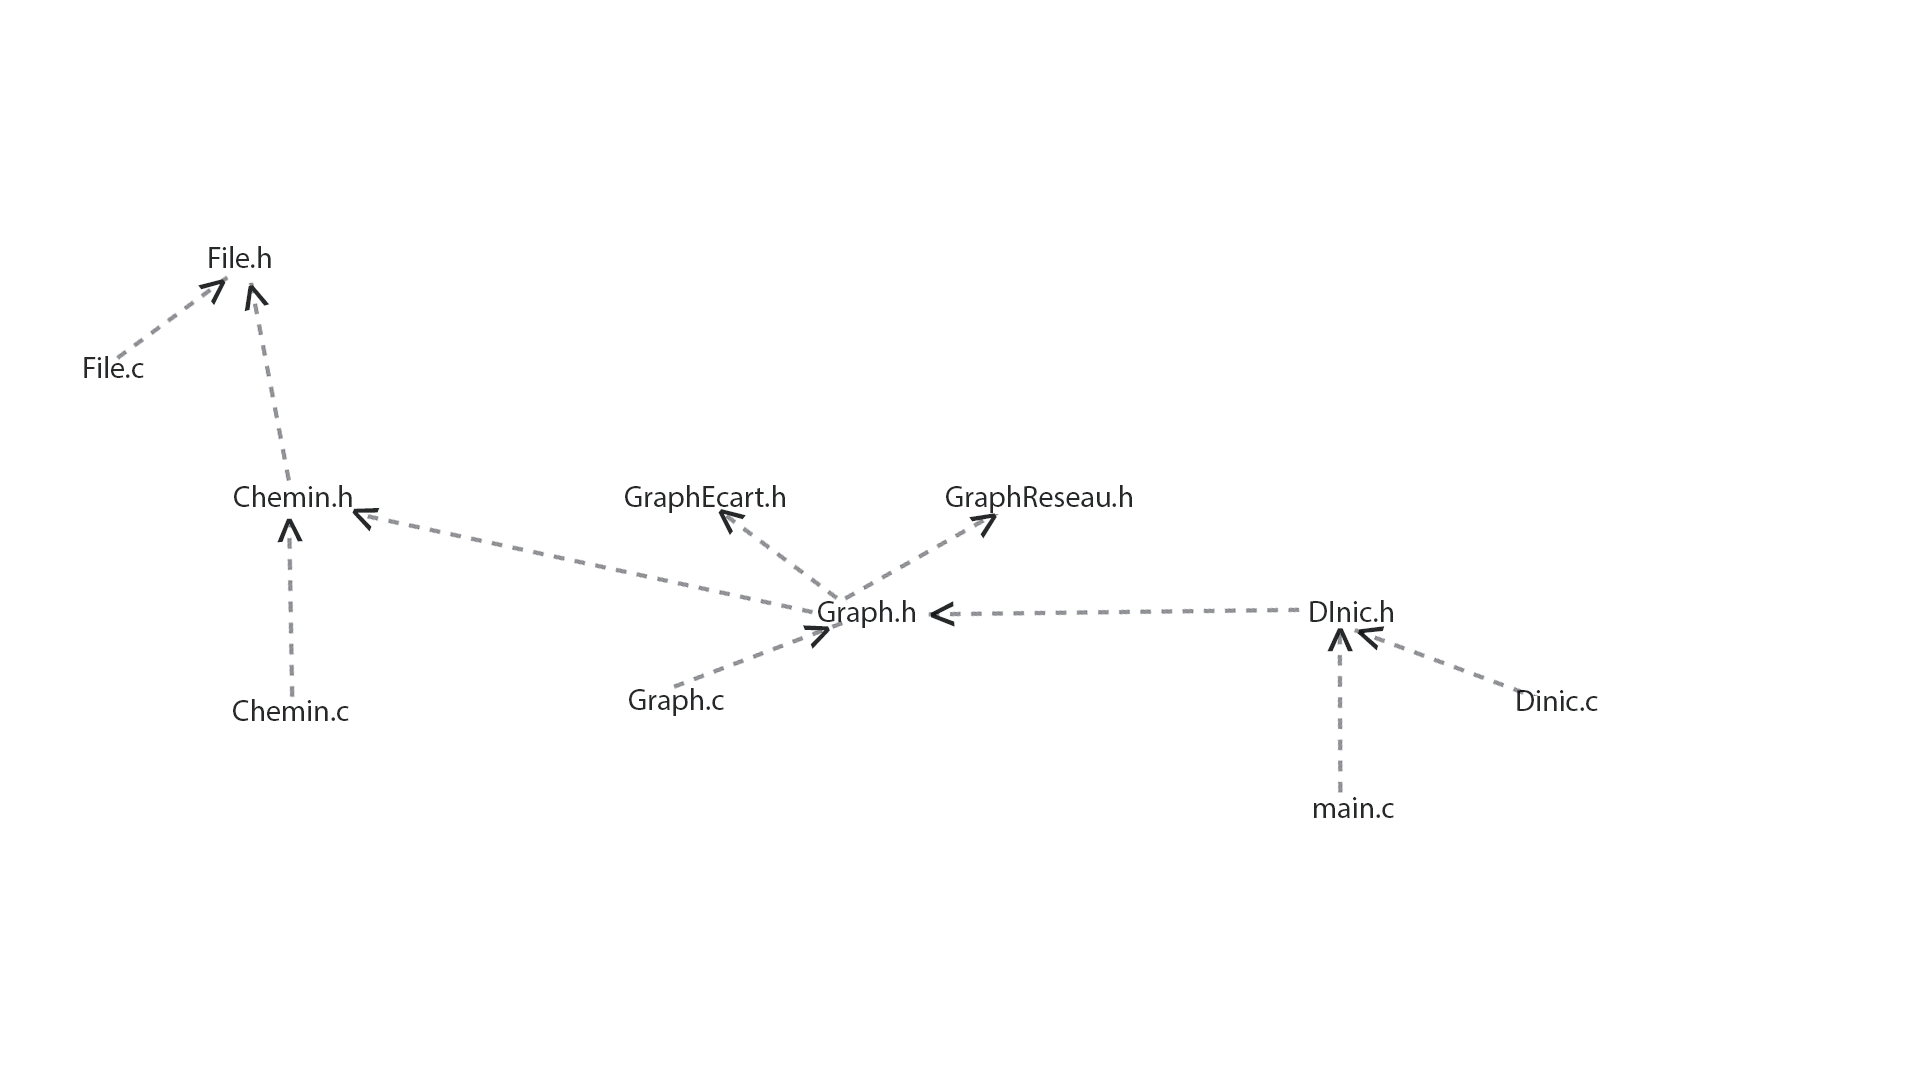
\includegraphics[width=1.2\textwidth]{images/fichiers.png}\\

	La descritpion de la file ainsi que les déclarations des fonctions applicables dessus se trouvent dans le ficher \verb|File.h| et ses fonctions sont décrites dans le fichier \verb|File.c|.

	Le réseau et le graphe d'écart sont tout deux des graphes et le chemin est construit à partir d'un graphe donc les fonctions dépendant de ces 3 structures de données sont contenues dans le ficher \verb|Graph.c|. Ce dernier importe 4 fichiers d'entête : \verb|GraphReseau.h|, \verb|GraphEcart.h| et \verb|Chemin.h| contenant la description des structures de données respectives. Le dernier fichier importé est \verb|Graph.c|, contenant la déclaration des fonctions produites dans le fichier \verb|Graph.c|.

	Enfin, \verb|Dinic.h| contient la signature de la fonction programmée dans le fichier \verb|Dinic.c|, et \verb|main.c| fait tourner le programme et maximise le flot du réseau donné en paramètres.

	Ainsi, la File est importée dans le Chemin pour permettre de trouver le plus court chemin, le Chemin, le Graphe Écart et le Réseau sont importés dans le Graphe, le Graphe est importé dans Dinic et enfin Dinic est importé dans le main.

	\verb|File.h| étant importé par tout les autres fichiers directement ou indirectement, toutes les inclusions de librairies sont faites dans ce fichier.

	\chapter{Mode d'emploi}

	L'entrée du programme est un fichier contenant la description d'un réseau au format \textbf{DIMACS}. (des exemples de ce format sont présents dans le dossier \verb|./DIMACS/| ou encore sur \verb*|MOODLE|).

	On va donc exécuter notre programme sur ce réseau pour maximiser le flot et obtenir un nouveau fichier $result.txt$ en sortie, contenant la description du réseau de flot maximum ainsi que le flot maximum final.

	Pour lancer le programme, un \verb|MAKEFILE| est mis à disposition pour gérer la compilation. La compilation se résume donc à lancer un terminal dans le répertoir courant et lancer la commande \verb|make|. Cette commande exécute les commandes de compilation et liens avec les options \verb|-Wall| et \verb|-g|. On obtient ainsi tout les warnings et on peut lancer le programme sous un débogueur comme \verb|gdb|. Le compilateur utilisé est \verb|gcc|. L'exécutable produit est \verb|a.out|.

	Le programme nécessite un fichier en entrée, fournissant le réseau initial. Il faut saisir les chemin et le nom du fichier en question. On peut donc exécuter les lignes suivantes :
	\lstset{language=bash}
	\begin{lstlisting}
		make
	\end{lstlisting}
	Commande compilant et faisant les liens d'import. Un fichier `a.out` exécutable est généré. Le programme peut être lancé par exemple des différentes manières suivantes :

	\begin{lstlisting}
		./a.out
		DIMACS/net1.txt
	\end{lstlisting}
	Le fichier `result.txt` contient à présent le réseau à 5 sommets de flot maximum.

	\begin{lstlisting}
		./a.out
		DIMACS/net2.txt
	\end{lstlisting}
	Le fichier `result.txt` contient à présent le réseau à 6 sommets de flot maximum.

	\begin{lstlisting}
		./a.out
		DIMACS/G_100_300.max
	\end{lstlisting}
	Le fichier `result.txt` contient à présent le réseau à 102 sommets de flot maximum.

	\begin{lstlisting}
		./a.out
		DIMACS/G_900_2700.max
	\end{lstlisting}
	Le fichier `result.txt` contient à présent le réseau à 902 sommets de flot maximum.

	\begin{lstlisting}
		./a.out
		DIMACS/G_2500_7500.max
	\end{lstlisting}
	Le fichier `result.txt` contient à présent le réseau à 2502 sommets de flot maximum.

	Les fonctions \verb|buildGraph|, \verb|buildRG|, \verb|shortestPath|, \verb|minCapa|, \verb|updateFlowInRG|, \verb|updateFlowInNet|, \verb|dinic| et \verb|main| sont décrites en pseudo-code dans un autre fichier.




	\chapter{Description des exemples traités}

	Tous les fichiers de graphes fournis se trouvent actuellement dans le répertoire \textbf{DIMACS}.

	Tous les fichiers ayant été donnés ont été traités. Les résultats obtenus sont les suivants :
	\begin{itemize}
        \item net1.txt : flot maximum = 40.
        \item net2.txt : flot maximum = 15.
        \item G\_100\_300.max : flot maximum = 9860177.
        \item G\_900\_2700.max : flot maximum = 28258807.
        \item G\_2500\_7500.max : flot maximum = 42791871.
	\end{itemize}

	Les résultats sont bien ceux souhaités.


	\chapter*{Conclusion}
	\pagenumbering{Alph}
	
	Le projet nous a permis de consolider nos connaissances en $C$, structures de données, algorithmes de parcours de graphes et maximisation de flot dans un réseau.
	
	Nos principales difficultés venaient d'une erreur d'inattention.
	
	Cependant, en travaillant à deux et en demandant un peu d'aide à un enseignant, nous avons finis par résoudre cette erreur et notre programme fonctionne pour tout réseau à maximiser et des fichiers ayant un format pas nécessairement strictement identiques.
	
	

	\chapter{Améliorations Possibles :}

	On remarque qu'au niveau de la structuration des structres, on peut améliorer et garder une structure globale pour un sommet et contruire des graphs différents en fonction de cela.

	On pense également que notre structure est plus claire et compréhensible que d'autres structures moins coteuses en termes de mémoire.

	Mais au niveau du traîement, nous avons essayés de ne pas faire de parcours inutil et nous avons ajoutés des conditions pour éviter des parcours inutiles.



	 \chapter{Technique :}

	 Nous avons utilisés $Git$ pour gérer notre projet, ce qui nous a permis de travailler plus efficacement. Techiniquement, on a pas eu de contraintes.

	\chapter*{Bilan personnel}
	
	On tient à remercier Monsieur Julien Forget de nous avoir données des pistes pour corriger des erreurs. À travers ce projet, nous avons améliorés nos conaissances sur les poiteurs et le parcours des graphes. Nous avons également enrichis nos compétences en programmation $C$ avancé et la compréhension des algorithmes de parcours.
	
	On a essayés de créer des tableaux dynamique qui nous permettent de faire fonctionner l'algorithme sur n'importe quel ficher de n'importe quelle taille de graphe.
	
	Notre méthode de travail était efficace étant donné que nous avons tous les deux essayés de répondre au probleme séparement et avons réalisés le déboguing ensemble. Nous n'avons pas répartis les tâches, nous avons répartis les algorithmes à programmer. Cependant, le déboguing a été fait ensemble, ce qui nous a fait gagner beaucoup de temps.

\end{document}
